\begin{figure*}
\centering
  \begin{tabular}{ccc}
%%%%% expt1  
  \begin{subfigure}{0.32\textwidth}
 \tabl{c}{\scalebox{0.6}{\begin{tikzpicture}
      \begin{axis}[
	xlabel={timestep},
	ylabel={Cumulative regret},
       clip mode=individual,grid,grid style={gray!30},
  legend style={at={(0.5,-0.2)},anchor=north,legend columns=3} ]  
  % UCB    

\addplot table[x index=0,y index=1,col sep=tab,each nth point={10}] {results/Expt1/UCB_Vcomp_subsampled.txt};
\addplot table[x index=0,y index=1,col sep=tab,each nth point={10}] {results/Expt1/DMEDcomp_subsampled.txt};
\addplot table[x index=0,y index=1,col sep=tab,each nth point={10}] {results/Expt1/KLUCBcomp_subsampled.txt};
\addplot table[x index=0,y index=1,col sep=tab,each nth point={10}] {results/Expt1/MOSScomp_subsampled.txt};
\addplot table[x index=0,y index=1,col sep=tab,each nth point={10}] {results/Expt1/UCB1comp_subsampled.txt};
\addplot table[x index=0,y index=1,col sep=tab,each nth point={10}] {results/Expt1/TScomp_subsampled.txt};
\addplot table[x index=0,y index=1,col sep=tab,each nth point={10}] {results/Expt1/EclUCB01comp_subsampled.txt};
      \legend{UCB-V,DMED,KL-UCB,MOSS,UCB1,TS,EClusUCB(p=4)}
      \end{axis}
      \end{tikzpicture}}\\}
			\caption{Experiment $1$: $20$ Bernoulli-distributed arms with $r_{i_{{i}\neq {*}}}=0.07$ and $r^{*}=0.1$.}
  \label{fig:1}
  \end{subfigure}
	&
	%%%%%%% Expt 2
	  \begin{subfigure}{0.32\textwidth}
 \tabl{c}{\scalebox{0.6}{\begin{tikzpicture}
      \begin{axis}[
	xlabel={timestep},
	ylabel={Cumulative regret},
       clip mode=individual,grid,grid style={gray!30},
  legend style={at={(0.5,-0.2)},anchor=north,legend columns=3} ]
      % UCB
\addplot table[x index=0,y index=1,col sep=tab,each nth point={10}] {results/Expt2/UCB1comp_subsampled.txt};
\addplot table[x index=0,y index=1,col sep=tab,each nth point={10}] {results/Expt2/clucb_p_10_comp_subsampled.txt};
\addplot table[x index=0,y index=1,col sep=tab,each nth point={10}] {results/Expt2/Med_Elimcomp_subsampled.txt};
\addplot table[x index=0,y index=1,col sep=tab,each nth point={10}] {results/Expt2/UCB_Improvedcomp_subsampled.txt};
\addplot table[x index=0,y index=1,col sep=tab,each nth point={10}] {results/Expt2/MOSScomp_subsampled.txt};
\addplot table[x index=0,y index=1,col sep=tab,each nth point={10}] {results/Expt2/EclUCB01_comp_subsampled.txt};
      \legend{UCB1,ClusUCB(p=10),Med-Elim,UCB-Improved,MOSS,EClusUCB(p=10)}
      \end{axis}
      \end{tikzpicture}}\\}
			\caption{Experiment $2$: $100$ Gaussian-distributed arms with $r_{i_{{i}\neq {*}:1-33}}=0.01$, $r_{i_{{i}\neq {*}:34-99}}=0.06$ and $r^{*}_{i=100}=0.1$.}
  \label{fig:2}
  \end{subfigure}
	&
	%%%%%%% Expt 3
	  \begin{subfigure}{0.32\textwidth}
 \tabl{c}{\scalebox{0.6}{\begin{tikzpicture}
      \begin{axis}[
	xlabel={Arms},
	ylabel={Cumulative regret},
       clip mode=individual,grid,grid style={gray!30},
  legend style={at={(0.5,-0.2)},anchor=north,legend columns=-1} ]
      % UCB
%\addplot table[x index=0,y index=1,col sep=tab] {results/Expt3/clUCB20_500.txt};
\addplot table[x index=0,y index=1,col sep=tab] {results/Expt3/clUCB20_500_1.txt};
\addplot table[x index=0,y index=1,col sep=tab] {results/Expt3/MOSS20_500.txt};
      \legend{ClusUCB(p=K/10),MOSS}
      \end{axis}
      \end{tikzpicture}}\\}
			\caption{Experiment $3$: $20$ to $500$ Bernoulli-distributed arms with $r_{i_{{i}\neq {*}}}=0.05$ and $r^{*}=0.1$.}
  \label{fig:3}
  \end{subfigure}
  \end{tabular}
\caption{Cumulative regret for various bandit algorithms on three stochastic K-armed bandit environments. 
}
\label{fig:karmed}
\end{figure*}



%\begin{figure}[!tbp]
%\label{fig:1}
%\begin{minipage}[b]{0.5\textwidth}
%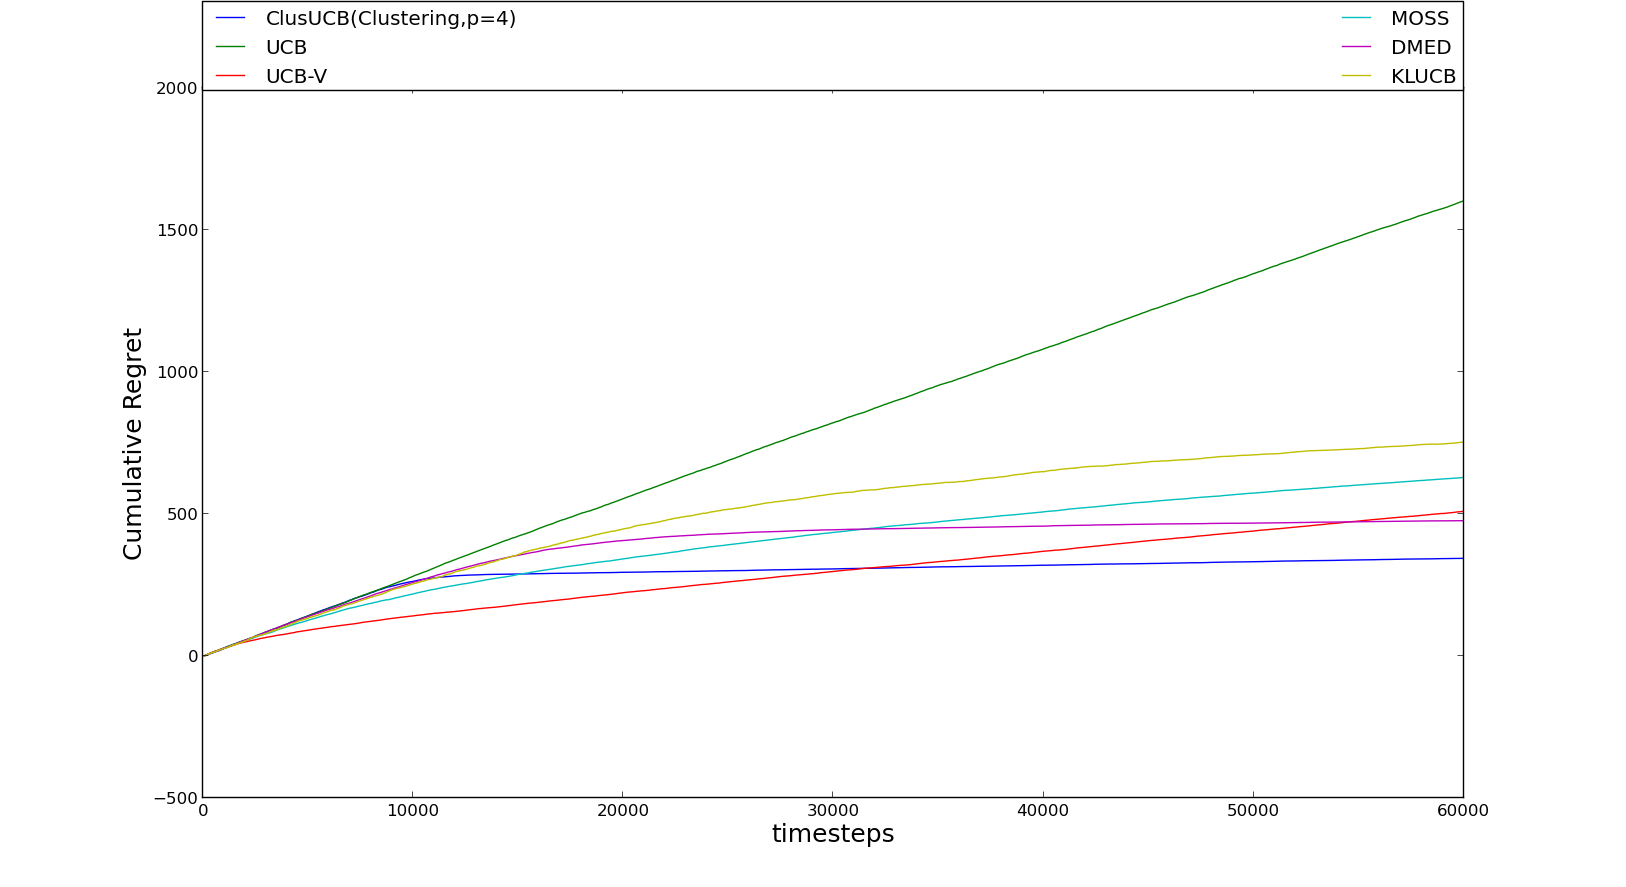
\includegraphics[width=\textwidth]{img/ClusUCB_variousAlgo.png}
%
%\caption{Experiment 1: Regret for various Algorithms. $T=60000$}
%\end{minipage}
%\end{figure}
%
%\hspace{0.1em}
%
%\begin{figure}[!tbp]
%\label{fig:2}
%\begin{minipage}[b]{0.5\textwidth}
%
%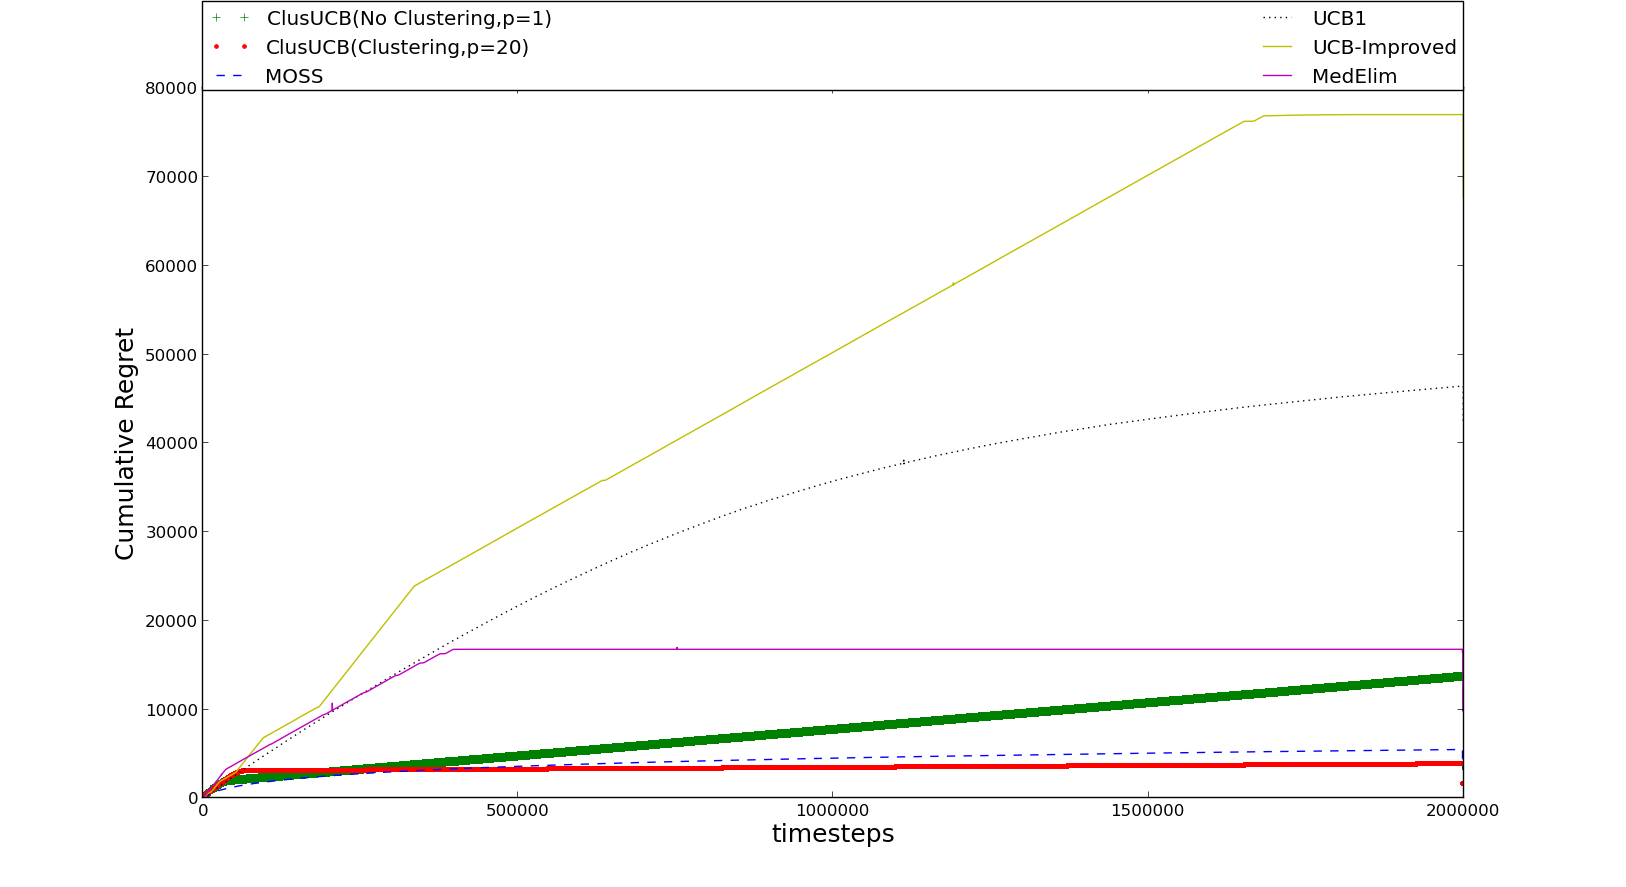
\includegraphics[width=\textwidth]{img/clusUCB_variousAlgo(expt2)_Final.png}
%\caption{Experiment 2: Regret for various Algorithms. $T=2\times 10^{6}$}
%\end{minipage}
%\end{figure}
%
%\hspace{0.1em}
%
%\begin{figure}[!tbp]
%\label{fig:3}
%\begin{minipage}[b]{0.5\textwidth}
%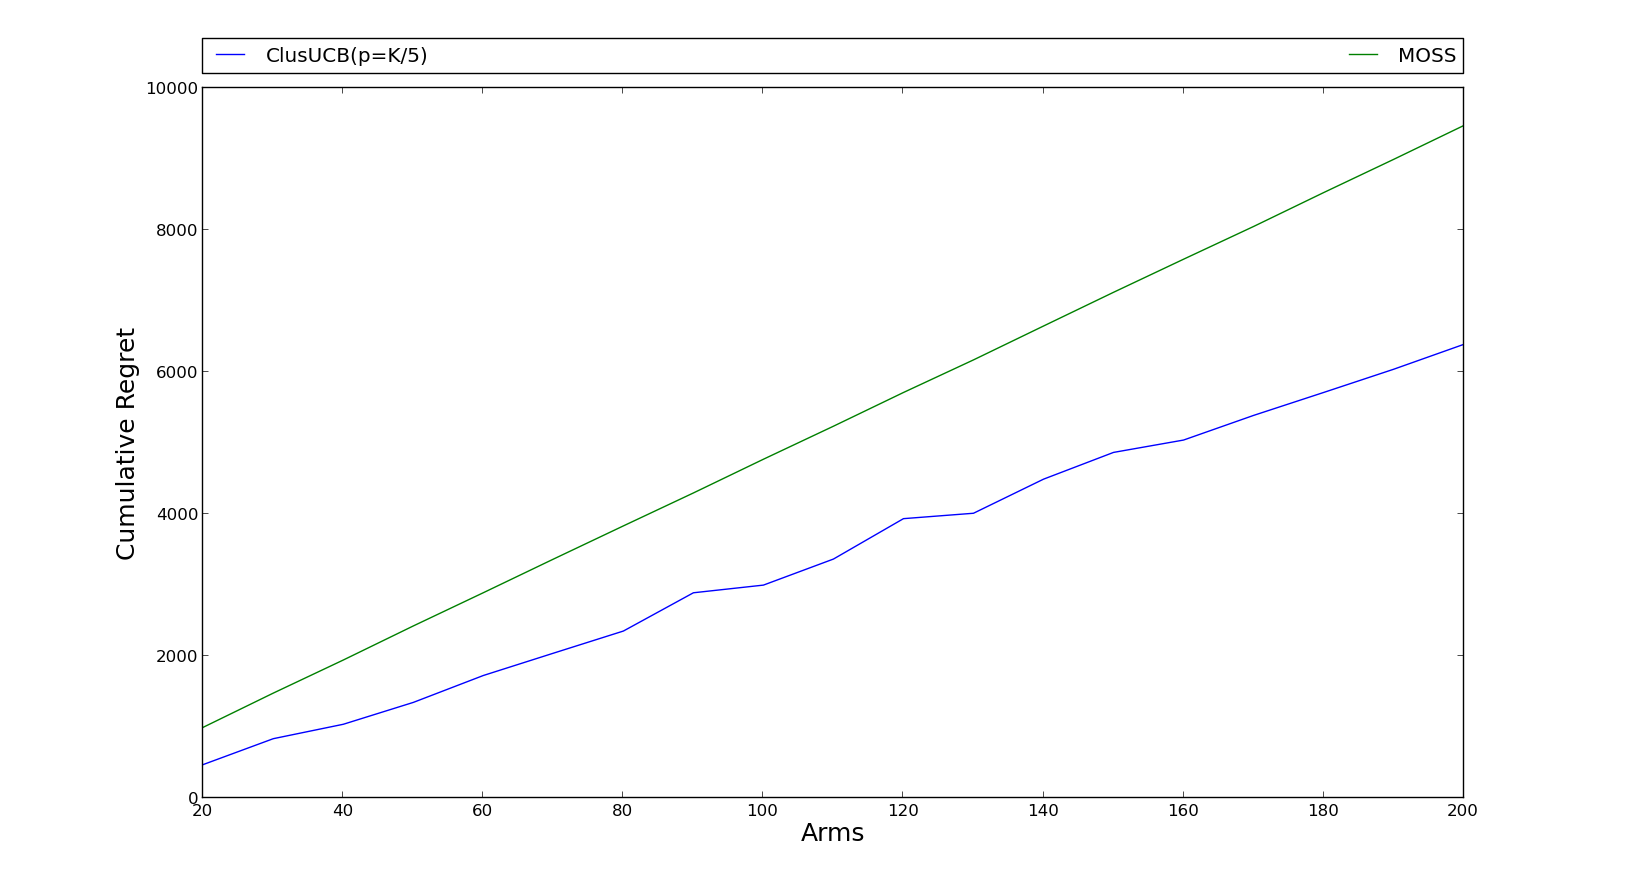
\includegraphics[width=\textwidth]{img/clUCB_MOSS_expt3.png}
%\caption{Experiment 3: Regret Growth for ClusUCB and MOSS . $T=10^{5} + K^{2}\times 10^{4}$ for $K=20$ to $200$}
%\end{minipage}
%\end{figure}
%
%\hspace{0.1em}
%


%In the stochastic bandit literature there are several powerful algorithms with and without proven regret bounds. Algorithms like $\epsilon$-greedy(\cite{sutton1998reinforcement}) or softmax(\cite{sutton1998reinforcement}) or UCB-Tuned(\cite{auer2002finite}) has no proven regret bounds. Again algorithms like UCB-$\delta$(\cite{abbasi2011improved}) with proven regret bound better than UCB1  falls within the realm of fixed confidence setting whereas one has to provide the probability of error $\delta$. We also make a distinction between frequentist based approach like the UCB algorithms and the Bayesian approach like the Thompson Sampling(\cite{agrawal2011analysis}). 
For the purpose of performance comparison using cumulative regret as the metric, we implement the following algorithms:  KL-UCB\cite{garivier2011kl}, DMED\cite{honda2010asymptotically}, MOSS\cite{audibert2009minimax}, UCB1\cite{auer2002finite}, UCB-Improved\cite{auer2010ucb}, Median Elimination\cite{even2006action}, Thompson Sampling(TS)\cite{agrawal2011analysis} and UCB-V\cite{audibert2009exploration}\footnote{The implementation for KL-UCB and DMED were taken from \cite{CapGarKau12}}. The parameters of ClusUCB algorithm for all the experiments are set as follows: $\psi=\log T$, $\rho_{s}=0.5$ and $\rho_{a}=0.25$. When $K$ is large and $p$ is small it is advantageous to run $\rho_{a} < \rho_{s}$(see 
Corollary \ref{Result:Corollary:2}) because this will aggressively eliminate arms within each cluster while full cluster elimination will be more conservative.
%So in all the experiments $\rho_{a}$ and $\rho_{s}$ are initialized to $1$ and then reduced after every round. By this definition of $\rho_{a},\rho_{s}$ we have made sure that their value always remain bounded $\in(0,1]$. 
% The intuition here is that since each cluster contains a large number of arms it should be eliminated less aggressively. 
%For parameter settings of ClusUCB and further experiments see Appendix \ref{App:Further:Expt}.

The first experiment is conducted over a testbed of $20$ arms for the test-cases involving Bernoulli reward distribution with expected rewards of the arms $r_{i_{{i}\neq {*}}}=0.07$ and $r^{*}=0.1$. These type of cases are frequently encountered in web-advertising domain. The horizon $T$ is set to $60000$. After limited exploratory experimentation the number of clusters $p$ for ClusUCB is set to $4$. The regret is averaged over $100$ independent runs and is shown in Figure \ref{fig:1}. EClusUCB, MOSS, UCB1, UCB-V, KL-UCB, TS and DMED are run in this experimental setup and we observe that EClusUCB performs better than all the aforementioned algorithms except TS. Because of the short horizon $T$, we do not implement UCB-Improved and Median Elimination on this test-case. We also observe that in this case the cumulative regret of EClusUCB and TS are almost similar to each other.

	The second experiment is conducted over a testbed of $100$ arms involving Gaussian reward distribution with expected rewards of the arms $r_{i_{{i}\neq {*}:1-33}}=0.01$, $r_{i_{{i}\neq {*}:34-99}}=0.06$ and $r^{*}_{i=100}=0.1$ with variance set at $\sigma^{2} = 0.3,\forall i\in A$. The horizon $T$ is set for a large duration of $2\times 10^{6}$ and the number of clusters $p=20$. The regret is averaged over $100$ independent runs and is shown in Figure \ref{fig:2}. In this case, in addition to EClusUCB, we also show the performance of ClusUCB algorithm (with $p=10$). From the results in Figure \ref{fig:2}, we observe that EClusUCB with $p=10$ outperforms ClusUCB with $p=10$ as well as MOSS, UCB1, UCB-Improved and Median-Elimination($\epsilon=0.03,\delta=0.1$). But as shown in Theorem \ref{Result:Theorem:1}, ClusUCB is better than UCB-Improved even though both are round based methods. Also the performance of UCB-Improved is poor in comparison to other algorithms, which is probably because of pulls wasted in initial exploration whereas ClusUCB with the choice of $\psi, \rho_{a}$ and $\rho_{s}$ performs much better.

	The third experiment is conducted over a testbed of $20-500$ (interval of $10$) arms with Bernoulli reward distribution, where the expected rewards of the arms are $r_{i_{{i}\neq {*}}}=0.05$ and $r^{*}=0.1$. The horizon $T$ is set to $10^{5} + K^{2}\times 10^{4}$ and the number of arms are increased from $K=20$ to $500$. The proposed algorithm ClusUCB is run with $p=K/10$. The regret is averaged over $500$ independent runs and is shown in Figure \ref{fig:3}. We report the performance of MOSS and ClusUCB only over this setup. From the results in Figure \ref{fig:3}, it is evident that the growth of regret for ClusUCB is lower than that of MOSS. 
%\begin{figure}
%\centering
%  \begin{tabular}{c}
%  %&
%  %%%%%%Expt4
%  \begin{subfigure}{0.45\textwidth}
% \tabl{c}{\scalebox{0.7}{\begin{tikzpicture}
%      \begin{axis}[
%	xlabel={timestep},
%	ylabel={Cumulative regret},
%       clip mode=individual,grid,grid style={gray!30},
%  legend style={at={(0.5,-0.2)},anchor=north, legend columns=4} ]
%      % UCB
%\addplot table[x index=0,y index=1,col sep=tab,each nth point={10}] {results/Expt4/clUCB1comp_subsampled.txt};
%\addplot table[x index=0,y index=1,col sep=tab,each nth point={10}] {results/Expt4/clUCB2comp_subsampled.txt};
%\addplot table[x index=0,y index=1,col sep=tab,each nth point={10}] {results/Expt4/clUCB3comp_subsampled.txt};
%\addplot table[x index=0,y index=1,col sep=tab,each nth point={10}] {results/Expt4/MOSScomp_subsampled.txt};
%\addplot table[x index=0,y index=1,col sep=tab,each nth point={10}] {results/Expt4/clUCB4comp_subsampled.txt};
%\addplot table[x index=0,y index=1,col sep=tab,each nth point={10}] {results/Expt4/clUCB5comp_subsampled.txt};
%\addplot table[x index=0,y index=1,col sep=tab,each nth point={10}] {results/Expt4/TScomp_subsampled.txt};
%      \legend{ClusUCB(1A),ClusUCB(4B),ClusUCB(10B),MOSS,ClusUCB(5S),ClusUCB(10S),TS}
%      %\legend{ClusUCB (NC, p=1),ClusUCB (C, p=4),ClusUCB(C, p=10) ,MOSS, ClusUCB(C, p=5, NAE), ClusUCB(C, p=10, NAE)}
%      %\legend{ClusUCB(1,A),ClusUCB(4,B),ClusUCB(10,B), MOSS,ClusUCB(5,S), ClusUCB(10,A)}
%      \end{axis}
%      \end{tikzpicture}}\\}
%			\caption{Experiment $4$: Cumulative regret for ClusUCB variants: $1,4,5,10$ correspond to number $p$ of clusters and A, S, B correspond to having only arm elimination, only cluster elimination and having both in Algorithm \ref{alg:clusucb}. For using just cluster elimination in ClusUCB, we stop when we left with only one cluster and play the max payoff arm of that cluster for the remaining time horizon. }
%  \label{Fig:variousClus}
%  \end{subfigure}
%  \end{tabular}
%\end{figure}

\begin{figure}
\centering
  \begin{tabular}{c}
  %&
  %%%%%%Expt4
  \begin{subfigure}{0.45\textwidth}
 \tabl{c}{\scalebox{0.7}{\begin{tikzpicture}
      \begin{axis}[
	xlabel={timestep},
	ylabel={Cumulative regret},
       clip mode=individual,grid,grid style={gray!30},
  legend style={at={(0.5,-0.2)},anchor=north, legend columns=4} ]
      % UCB
\addplot table[x index=0,y index=1,col sep=tab,each nth point={10}] {results/Expt4_1/clucb1_comp_subsampled.txt};
\addplot table[x index=0,y index=1,col sep=tab,each nth point={10}] {results/Expt4_1/clucb3_comp_subsampled.txt};
\addplot table[x index=0,y index=1,col sep=tab,each nth point={10}] {results/Expt4_1/clucb5_comp_subsampled.txt};
\addplot table[x index=0,y index=1,col sep=tab,each nth point={10}] {results/Expt4_1/clucb10_comp_subsampled.txt};
\addplot table[x index=0,y index=1,col sep=tab,each nth point={10}] {results/Expt4_1/clucb15_comp_subsampled.txt};
\addplot table[x index=0,y index=1,col sep=tab,each nth point={10}] {results/Expt4_1/clucb25_comp_subsampled.txt};
      \legend{ClusUCB(1),ClusUCB(3),ClusUCB(5),ClusUCB(10),ClusUCB(15),ClusUCB(25)} 
      %\legend{ClusUCB (NC, p=1),ClusUCB (C, p=4),ClusUCB(C, p=10) ,MOSS, ClusUCB(C, p=5, NAE), ClusUCB(C, p=10, NAE)}
      %\legend{ClusUCB(1,A),ClusUCB(4,B),ClusUCB(10,B), MOSS,ClusUCB(5,S), ClusUCB(10,A)}
      \end{axis}
      \end{tikzpicture}}\\}
			\caption{Experiment $4$: Cumulative regret for ClusUCB variants: $1,3,5,10,15,25$ correspond to number $p$ of clusters}
%and A, S, B correspond to having only arm elimination, only cluster elimination and having both in Algorithm \ref{alg:clusucb}. For using just cluster elimination in ClusUCB, we stop when we left with only one cluster and play the max payoff arm of that cluster for the remaining time horizon. 
  \label{Fig:variousClus}
  \end{subfigure}
  \end{tabular}
\end{figure}

	The fourth experiment is performed over a testbed having $50$ Gaussian-distributed arms with $r_{i_{:{{i}\neq {*}}}}=0.8,\forall i\in A$, $r^{*}=0.9$ and $\sigma^{2}=1.0$. In Figure \ref{Fig:variousClus}, we report the results with $T=400000$ averaged over $100$ independent runs for ClusUCB with  $p=\lbrace 1,3,5,10,15,25\rbrace$. Also, in this experiment we take $\psi = K^{2}T$, $\rho_a=0.25$ and $\rho_{s}=0.5$ as stated in Corollary \ref{Result:Corollary:2}. The high variance leads to a greater number of errors committed by ClusUCB-AE that is ClusUCB($p=1$) but as proved in Proposition \ref{proofTheorem:Prop:1} the cumulative regret is lesser than  ClusUCB. But because of the increased errors committed in predicting the optimal arm and because of the large horizon, we eventually see that ClusUCB(p=$5,10,25,25$) outperforms ClusUCB-AE while ClusUCB($p=3$) regret is worse than ClusUCB-AE. The error percentage in the $6$ cases (in the order as shown in legend of Fig \ref{Fig:variousClus}) are $14,12,5,3,3$ and $3$. The range of p is shown to be between $\sqrt{\log K}$ to $\frac{K}{2}$ and as we approach $\frac{K}{2}$ we see that the error percentage stabilizes to $3\%$.
	More experiments are shown in Appendix \ref{App:MoreExp}.
	
	
%	Two other benchmark algorithms are considered here, MOSS which is one of our main competitors and TS which has performed near equivalently in experiment $1$(see Fig \ref{fig:1}). In this case we see that, since $\rho_{a}$ is decreased very fast, the optimal arm $a^{*}$ gets eliminated most of the time for no clustering $p=1$. While a balance of $p,\rho_{a}$ and $\rho_{s}$ gives a much better result. ClusUCB with $p=4$ and $10$ 
%perform better than MOSS, while $p=1$ with just arm elimination does not converge and $p=5,10$ with just Cluster elimination and no arm elimination also does not converge, implying both cluster and arm elimination are necessary. This also concurs with the theoretical observations (see Proposition \ref{proofTheorem:Prop:2} and the discussion in Section \ref{sec:results} on the analysis of elimination error).
%Note also that ClusUCB($p=4$) outperforms TS in this setup.	
	
%We also see that in this testbed UCB-Improved performs the worst and it confirms our assumption that it spends too much pulls in the initial exploration.

%We set $\psi=1$, $\rho_{s}=\frac{1}{2^{m+1}}$ and $\rho_{a}=\frac{1}{2^{2m+1}}$.

%The jumps in the graph for ClusUCB happens because of the error(eliminating optimal arm) and the margin of error(in red) is also shown in the graph. 
%\todos{I did not see this jump in the txt files shared for Expt 3}
